\documentclass[letterpaper]{article}
\usepackage{amsmath}
\usepackage{algorithm}
\usepackage{multirow}
\usepackage{graphicx}

\begin{document}
\title{ECON 199 Problem Set 3}
\author{Will Koster (jameswk2; 651028726) \and Javier Garza (javierg2; 667146159)}
\date{Apr 10, 2020}
\maketitle

\clearpage

\begin{enumerate}
    \item \begin{enumerate}
            \item South Korea moves first because they undertake enough geopolitical risk to justify almost any action to the rest of the world. The United States moves next because it wants to make its decision with knowledge of the interests of South Korea. Then, North Korea gets to move. A compelling case could be made for North Korea moving first and last, but the outcome of the game would not change in that case. \\ 
                Each player can choose to be aggressive or passive. \\
                If everyone is aggressive, North Korea loses substantially. Their aggression justifies South Korea's, which justifies the United States', meaning that the latter two experience no negative diplomatic outcomes, while the economy and military of North Korea are severely damaged. \\
                If everyone is passive, North Korea receives aid from wealthy countries but it unable to build strength, but everyone else gets security at a very low cost. \\
                If North Korea is aggressive and everyone else is passive, North Korea does whatever it wants with no consequences, which is a win for them and a loss for everyone else. \\
                If South Korea is aggressive and everyone else is passive, North Korea looks oppressed, which is good for them, South Korea spends a bunch of money in exchange for a worse international reputation, and the United States gets brownie points from China. \\
                If the United States is aggressive and everyone else is passive, North Korea once again looks oppressed and gets enough help from China to sustain their economy, South Korea slightly suffers from the good fortune of North Korea, and the United States winds up in the doghouse with China (although the responsible American politicians likely benefit). \\
                If North Korea alone is passive, then they build justification for later aggression and get support from sympathetic governments around the world, and South Korea and the United States look like bullies. \\
                Is the United States alone is passive, South Korea's aggressiveness makes the United States look soft on authoritarianism (but improves its standing with China), North Korea experiences fewer roadblocks in improving their military, and South Korea is left to spend lots of money for minimal security. \\
                If South Korea alone is passive, South Korea experiences a substantial loss of domestic security but saves money, North Korea's military rise is largely thwarted, but not completely, and the United States is basically neutral. \\

                This leads to the following game tree. \\
                \hspace*{-2.2in}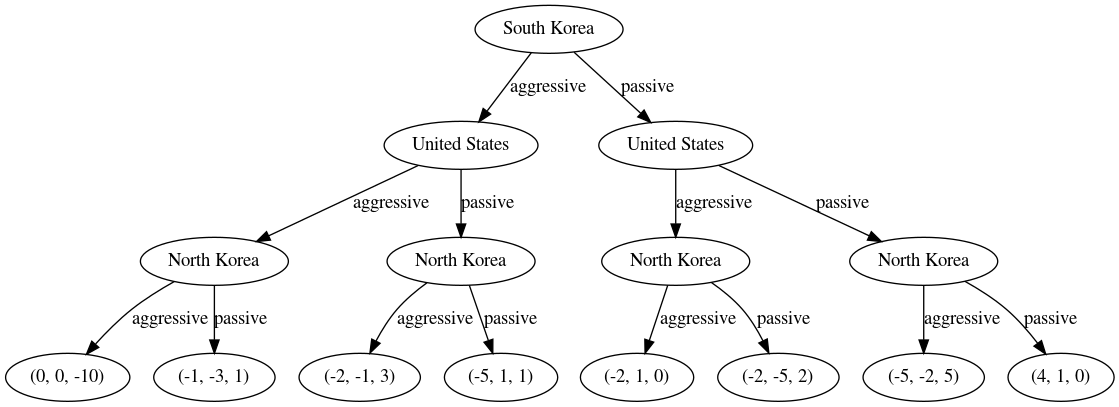
\includegraphics[scale=0.5]{tree} \\

                The rollback equilibrium is (aggressive, passive, aggressive). The United States should play passive no matter what South Korea does, meaning North Korea should play aggressive and South Korea should play aggressive.
            \item \begin{enumerate}
                    \item "Strategic patience" seems most similar to passive in this formulation of the game. 
                    \item Given the payoffs in the game above and assuming that other players play rationally, this is not an optimal strategic move. But one might also note that, if the United States always plays aggressive, this forces North Korea to always play passive. The downside to the United States comes not from North Korea's actions but from the ire of the international community and China specifically. If the government in the United States devalues those things, then aggressiveness might become a more reasonable strategy.
                \end{enumerate}
        \end{enumerate}
\end{enumerate}
\end{document}
